% Provenance (never printed): old premiere S material on the history of plate
% tectonics (from continental drift to seafloor spreading: the ridges, the
% magnetic stripes, the ages of the drilled floor); see
% sources/book2/PROVENANCE.md. Profiles are computed in
% figdata/grade-11/magnetic_stripes.py, the age map in seafloor_age.py, the
% drilling fit in sediment_ages.py.
\chapter{De la dérive des continents à l'expansion des fonds océaniques}\label{ch:g11:drift-to-spreading}

Au début des années 1950, au laboratoire Lamont de l'université Columbia,
une jeune géologue nommée Marie Tharp travaillait devant de longues rangées
de nombres. Chacun était une profondeur de l'Atlantique Nord, mesurée par
l'échosondeur d'un navire, l'une après l'autre le long de sa route. En les
reportant une à une, elle dessina la forme du fond océanique le long des
routes de navires qui avaient traversé l'océan. Au milieu de l'océan, le
fond s'élevait en une chaîne de montagnes --- et sur chaque route, le long
de la crête de cette chaîne, le fond replongeait dans une profonde
crevasse, comme si les montagnes avaient été fendues en leur milieu. Ce
chapitre montre comment de telles mesures du fond océanique ont fait d'une
idée rejetée, la dérive des continents, une théorie~: le fond océanique se
forme aux dorsales et s'en éloigne, et ses roches portent la trace de son
propre âge.
% ledger: aip:tharp, aip:featureless, usgs:echo-sounding

\begin{recall}
La dérive des continents est l'idée que les continents se déplacent~;
Alfred Wegener la défendit à partir de 1912 en s'appuyant sur l'ajustement
des côtes, les fossiles, les roches et les climats anciens, mais il ne put
dire ce qui les déplaçait. La surface de la Terre est faite de plaques
rigides, qui se rencontrent à des frontières divergentes, convergentes et
transformantes~; elles se déplacent de quelques centimètres par an, et
$\qty{1}{cm}$ par an font $\qty{10}{km}$
par million d'années (livre~1, année~7). Le fond océanique a son plateau
continental, ses plaines abyssales, ses dorsales et ses fosses (livre~1,
année~8). La Terre possède un champ magnétique, avec un pôle magnétique nord
et un pôle magnétique sud, que suit l'aiguille d'une boussole~; une
impulsion sonore envoyée dans l'eau revient sous forme d'écho au bout d'une
durée qui donne la distance (les livres de physique).
\end{recall}

\section{Pourquoi la dérive fut rejetée}

Les arguments de Wegener montraient que les continents avaient été réunis
autrefois. Ils ne montraient pas comment ils avaient pu se déplacer. Wegener
imaginait les continents labourant la roche du fond océanique, et les
physiciens répondirent qu'aucune force connue ne pouvait pousser un
continent à travers une roche solide sans l'écraser. Pendant un demi-siècle,
la plupart des géologues conclurent que les continents n'avaient pas bougé
du tout.
% ledger: usgs:wegener-1912, usgs:jeffreys (Book 1 rows)

Il manquait deux choses. La première était un mécanisme. La seconde, qui
mena à la première, était la connaissance du fond des océans, qui couvre la
plus grande partie de la surface terrestre et que, en 1912, presque personne
n'avait vu~: on le supposait être une plaine presque sans relief.
% ledger: aip:tharp, aip:featureless

\section{Cartographier le fond océanique}

Un échosondeur envoie une brève impulsion sonore depuis la coque d'un
navire vers le fond de la mer et chronomètre son écho. Le son se propage
dans l'eau de mer à environ \qty{1500}{m/s}~; l'impulsion descend et
remonte, si bien qu'un délai $t$ correspond à une profondeur
\[
  d = \frac{v\,t}{2}.
\]
Un délai de \qty{6.0}{s}, par exemple, correspond à $1500 \times 6.0/2 =
\qty{4500}{m}$ d'eau. Au \textsc{xix}\textsuperscript{e}~siècle, on mesurait
les profondeurs une à une, en descendant jusqu'au fond une ligne lestée.
Après la Première Guerre mondiale, les échosondeurs prirent le relais, et
les enregistrements de leurs échos révélèrent un fond bien plus accidenté
qu'on ne le pensait~; dans les années 1950, des campagnes de navires de
nombreux pays montrèrent qu'une grande chaîne de montagnes sous-marine fait
presque le tour complet de la Terre.
% ledger: noaa:sound-seawater, usgs:echo-sounding, usgs:line-soundings

\begin{history}[Marie Tharp et la vallée du rift, 1952]
% ledger: aip:tharp, aip:featureless
À partir de 1947, le géophysicien Bruce Heezen avait rassemblé des profils
d'échosondage à travers l'Atlantique Nord. Marie Tharp, qui n'avait pas le
droit d'embarquer sur les navires de recherche à l'époque, transforma ce
qu'elle appela plus tard «~d'interminables rangées de chiffres de sondage~»
en dessins du fond de la mer. En 1952, en rangeant dans l'ordre du nord au
sud les routes orientées est--ouest, elle vit qu'un trait s'alignait d'une
route à l'autre~: une crevasse le long de la crête de la dorsale
médio-atlantique, une vallée de rift. Heezen crut d'abord à une erreur.
Puis on découvrit que les épicentres des séismes de l'Atlantique, reportés
à la même échelle, tombaient dans la vallée du rift elle-même. La carte du
fond des océans du monde de Tharp et Heezen, peinte par l'artiste Heinrich
Berann en 1977, donna au public la première image réaliste du fond
océanique~; en 1997, la bibliothèque du Congrès la compta parmi les quatre
grands cartographes du \textsc{xx}\textsuperscript{e}~siècle.
\end{history}

Les dorsales médio-océaniques forment un seul système, presque continu,
long d'environ \qty{65000}{km}, dont plus des neuf dixièmes sont sous
l'eau~; la crête se trouve en moyenne à \qty{2500}{m} sous la surface. Le
long de la dorsale médio-atlantique, lente, la crête est entaillée par une
vallée de rift~; le long de la dorsale du Pacifique Est, plus rapide, c'est
un sommet lisse et doux. Les séismes des océans suivent étroitement les
dorsales. Tout désignait la dorsale comme un lieu où il se passait quelque
chose --- mais quoi~?
% ledger: noaa:ridge, aip:tharp

\section{L'expansion des fonds océaniques}

\begin{history}[Hess et le tapis roulant, 1962]
% ledger: usgs:hess, hess:1962
En 1962, Harry Hess, géologue à l'université de Princeton et amiral de la
réserve de la marine, publia \emph{History of Ocean Basins}.
Il proposait que de la roche chaude monte sous les dorsales et devienne un
nouveau fond océanique, qui s'éloigne ensuite des deux côtés comme un tapis
roulant, et replonge dans le manteau au niveau des fosses. Robert Dietz,
arrivé à la même idée, lui donna son nom~: l'\omterm{def:g11:drift-to-spreading:spreading}{expansion des fonds
océaniques}. L'idée expliquait pourquoi la Terre ne grossit pas bien qu'un
fond nouveau se forme sans cesse, pourquoi si peu de sédiments reposent sur
le fond océanique, et pourquoi les roches du fond océanique sont bien plus
jeunes que celles des continents.
\end{history}

\begin{definition}[Expansion des fonds océaniques]\label{def:g11:drift-to-spreading:spreading}
L'\emph{expansion des fonds océaniques}\index{expansion des fonds oceaniques@expansion des fonds océaniques}
est le processus par lequel un
nouveau fond océanique se forme le long de la crête d'une dorsale
médio-océanique, où de la roche fondue monte du manteau et se solidifie,
puis s'éloigne de la dorsale des deux côtés, si bien que le fond océanique
vieillit avec la distance à la dorsale.
\end{definition}

\begin{definition}[Vitesse d'expansion]\label{def:g11:drift-to-spreading:spreading-rate}
La \emph{vitesse d'expansion totale}\index{vitesse d'expansion} d'une
dorsale est la vitesse à laquelle s'écartent les deux plaques situées de
part et d'autre. La \emph{demi-vitesse d'expansion} est la vitesse à
laquelle le fond d'un côté s'éloigne de l'axe de la dorsale. Quand
l'expansion est symétrique, la vitesse totale vaut deux fois la
demi-vitesse.
\end{definition}

Les dorsales s'ouvrent à des vitesses très différentes. La dorsale
médio-atlantique s'ouvre de \qtyrange{2}{5}{cm} par an, la dorsale du
Pacifique Est de \qtyrange{6}{16}{cm} par an. Du fond océanique qui existe
aujourd'hui, environ un tiers a été formé à des dorsales lentes (vitesses
totales de \qtyrange{20}{55}{mm} par an) et environ deux cinquièmes à des
dorsales rapides (\qtyrange{75}{180}{mm} par an).
% ledger: noaa:ridge, seton:rate-classes

L'idée de Hess était audacieuse, et elle n'avait d'abord guère de preuves
directes. Les preuves vinrent de deux directions inattendues~: le magnétisme
du fond océanique et ses sédiments.

\section{Les inversions magnétiques et le fond océanique rayé}

\subsection{Une roche garde la mémoire du champ}

Le basalte du fond océanique contient de petits grains de magnétite, un
oxyde de fer fortement magnétique. Quand la lave basaltique sort, elle est
bien trop chaude pour garder une aimantation durable~; en refroidissant,
les grains s'aimantent parallèlement au champ terrestre qui les entoure, et
cette direction se fige alors dans la roche.
% ledger: usgs:magnetometers

\begin{definition}[Aimantation rémanente~; température de Curie]\label{def:g11:drift-to-spreading:remanence}
La \emph{température de Curie}\index{temperature de Curie@température de Curie}
d'un minéral magnétique est la température au-dessus de laquelle il
ne peut garder d'aimantation propre~: environ \qty{580}{\celsius} pour la
magnétite. Une roche dont les grains magnétiques refroidissent sous leur
température de Curie dans le champ terrestre garde une aimantation
parallèle au champ de cette époque, l'\emph{aimantation
rémanente}\index{aimantation remanente@aimantation rémanente}. Elle dure
longtemps après que le champ a changé, à moins que la roche ne soit de
nouveau chauffée au-dessus de la température de Curie.
\end{definition}
% ledger: tarduno:curie

\begin{omfigure}
\begin{tikzpicture}[font=\footnotesize, >={Stealth[length=5pt]}]
  % ground and lava flow
  \fill[lith basalt] (0,0) rectangle (11,0.6);
  \fill[omLithBasalt!45!red!35] (0,0.6) -- (11,0.6) -- (11,1.9) .. controls (9,2.0) and (4,2.15) .. (0,2.05) -- cycle;
  \fill[omLithBasalt!70] (0,1.35) -- (11,1.25) -- (11,1.9) .. controls (9,2.0) and (4,2.15) .. (0,2.05) -- cycle;
  \draw[black!60] (0,1.35) -- (11,1.25);
  \draw[line width=0.8pt] (0,2.05) .. controls (4,2.15) and (9,2.0) .. (11,1.9);
  \draw[black!60] (0,0.6) -- (11,0.6);
  % field lines (northern hemisphere: pointing down to the north)
  \foreach \x in {0.6,2.4,4.2,6.0,7.8,9.6} {
    \draw[->, omDef, line width=0.9pt] (\x,4.0) -- (\x+1.1,2.55);
  }
  \node[anchor=south west, text=omDef] at (0.2,4.05) {le champ magnétique terrestre};
  % locked grains in the cooled top
  \foreach \x in {0.5,1.3,...,10.5} {
    \draw[->, black, line width=0.6pt] (\x,1.86) -- (\x+0.25,1.53);
  }
  % random grains in the hot interior
  \foreach \x/\a in {0.6/20,1.5/140,2.3/250,3.2/80,4.0/310,4.9/190,5.7/40,6.6/120,7.4/280,8.3/20,9.1/200,10.0/330} {
    \draw[->, black!55, line width=0.5pt] (\x,0.95) -- ++(\a:0.22);
  }
  \node[anchor=west, align=left] at (11.15,1.75) {refroidie sous \qty{580}{\celsius}~: les\\grains orientés selon le champ};
  \node[anchor=west, align=left] at (11.15,0.92) {encore au-dessus de \qty{580}{\celsius}~:\\pas d'aimantation durable};
  \node[anchor=west, align=left] at (11.15,0.25) {roche plus ancienne};
  \node[anchor=west] at (9.0,4.25) {nord $\rightarrow$};
\end{tikzpicture}

{\small Une coulée de lave qui refroidit (schéma, hémisphère Nord, où le
champ pointe vers le nord et vers le bas). Le haut de la coulée est passé
sous la \omterm{def:g11:drift-to-spreading:remanence}{température de Curie} de la magnétite~: ses grains magnétiques
(flèches noires) gardent la direction du champ. L'intérieur, encore plus
chaud, n'enregistre encore rien~; il enregistrera le champ du moment où il
refroidira.}
\end{omfigure}

\subsection{Le champ s'inverse}

Au début du \textsc{xx}\textsuperscript{e}~siècle, Bernard Brunhes (en 1906)
puis Motonori Matuyama (dans les années 1920) découvrirent que les roches
volcaniques se rangent en deux groupes. Dans les unes, l'aimantation pointe
dans le même sens que le champ actuel~; dans les autres, elle pointe en sens
opposé, comme si les pôles magnétiques nord et sud avaient échangé leurs
places. Le champ lui-même s'était inversé, encore et encore.
% ledger: usgs:reversals

\begin{definition}[Inversion magnétique~; polarité normale et inverse]\label{def:g11:drift-to-spreading:reversal}
Une \emph{inversion magnétique}\index{inversion magnetique@inversion magnétique}
est un échange des pôles magnétiques nord et sud de la Terre.
Une époque où le champ pointait comme aujourd'hui est une époque de
\emph{polarité normale}\index{polarite normale@polarité normale}~; une
époque où il pointait en sens opposé, une époque de \emph{polarité
inverse}\index{polarite inverse@polarité inverse}. Une roche aimantée
pendant l'une ou l'autre époque a la même polarité.
\end{definition}

Des laves datées donnent la succession des intervalles normaux et
inverses~: l'\emph{échelle des inversions géomagnétiques}. Ses longs
intervalles portent le nom de scientifiques qui ont étudié le magnétisme
terrestre (Brunhes, Matuyama, Gauss, Gilbert)~; les courts événements qu'ils
contiennent, celui des lieux où on les a découverts.

\begin{omfigure}
\begin{tikzpicture}
\begin{axis}[width=0.92\linewidth, height=3.2cm, xmin=0, xmax=5.5, ymin=-0.9, ymax=1.9,
  axis y line=none, axis x line*=bottom, xtick={0,0.5,...,5.5}, tick label style={font=\small},
  xlabel={âge (millions d'années)}, label style={font=\small}, clip=false]
\addplot[fill=black, draw=none] table {figdata/out/grade-11-magnetic_stripes-timescale.dat};
\draw[black] (axis cs:0,0) rectangle (axis cs:5.5,1);
\begin{scope}[every node/.style={font=\scriptsize, anchor=south}]
  \node at (axis cs:0.39,1.05) {Brunhes};
  \node at (axis cs:1.68,1.05) {Matuyama};
  \node at (axis cs:3.08,1.05) {Gauss};
  \node at (axis cs:4.74,1.05) {Gilbert};
\end{scope}
\draw[black!60] (axis cs:0.78,1) -- (axis cs:0.78,1.45);
\draw[black!60] (axis cs:2.581,1) -- (axis cs:2.581,1.45);
\draw[black!60] (axis cs:3.58,1) -- (axis cs:3.58,1.45);
\begin{scope}[every node/.style={font=\scriptsize, anchor=north}]
  \node at (axis cs:1.03,-0.05) {Jaramillo};
  \node at (axis cs:1.86,-0.05) {Olduvai};
\end{scope}
\node[font=\scriptsize, anchor=west] at (axis cs:5.55,0.75) {normale};
\node[font=\scriptsize, anchor=west] at (axis cs:5.55,0.25) {(noir)};
\end{axis}
\end{tikzpicture}

{\small L'échelle des inversions géomagnétiques des 5.5 derniers millions
d'années~: en noir la \omterm{def:g11:drift-to-spreading:reversal}{polarité normale}, en blanc la \omterm{def:g11:drift-to-spreading:reversal}{polarité inverse}.
L'intervalle normal actuel a commencé il y a \num{780000}~ans~; il y a eu
vingt inversions au cours des cinq derniers millions d'années.
Données~: Cande et Kent (1995).}
\end{omfigure}
% ledger: ck95:chrons

\subsection{Des bandes sur le fond océanique}

À partir des années 1950, des navires remorquèrent des magnétomètres à
travers les océans, et découvrirent que le champ à la surface de la mer
n'était pas le champ régulier attendu du noyau terrestre~: il était un peu
plus fort ici, un peu plus faible là.
% ledger: usgs:magnetometers

\begin{definition}[Anomalie magnétique]\label{def:g11:drift-to-spreading:anomaly}
En un point de la surface de la mer,
l'\emph{anomalie magnétique}\index{anomalie magnetique@anomalie magnétique} est l'intensité mesurée du champ magnétique moins l'intensité
qu'on y attend du seul champ terrestre. Elle est positive là où les roches
sous-jacentes renforcent le champ, négative là où elles s'y opposent. Elle
est petite devant le champ lui-même, et se mesure en nanoteslas
(\unit{nT}).
\end{definition}

Cartographiées sur une vaste région, les anomalies dessinaient des bandes
parallèles à la crête de la dorsale, alternativement positives et
négatives, comme le pelage d'un zèbre --- et le motif d'un côté de la
dorsale était l'image miroir du motif de l'autre côté.
% ledger: usgs:magnetometers

\begin{history}[Vine et Matthews, 1963]
% ledger: vm:1963, usgs:magnetometers
En septembre 1963, Fred Vine et Drummond Matthews publièrent un court
article dans la revue \emph{Nature}, \emph{Magnetic anomalies over oceanic
ridges}. Ils y réunissaient l'expansion de Hess et les inversions du champ.
Si un nouveau fond se forme à la crête et s'en éloigne pendant que le champ
s'inverse, chaque bande de fond enregistre la polarité de l'époque où elle
a refroidi. Le fond devient une bande magnétique rayée, qui se déroule des
deux côtés de la dorsale~: anomalies positives au-dessus des bandes
normales, négatives au-dessus des bandes inverses, la même séquence des deux
côtés.
\end{history}

\begin{omfigure}
\begin{tikzpicture}
\begin{axis}[hide axis, axis equal image, width=0.94\linewidth, xmin=-320, xmax=420, ymin=-120, ymax=160, clip=false]
  % block faces
  \fill[white] (axis cs:-300,0) -- (axis cs:300,0) -- (axis cs:390,70) -- (axis cs:-210,70) -- cycle;
  \fill[omLithBasalt!25] (axis cs:-300,0) rectangle (axis cs:300,-60);
  \fill[omLithBasalt!45] (axis cs:300,0) -- (axis cs:390,70) -- (axis cs:390,10) -- (axis cs:300,-60) -- cycle;
  \addplot[fill=black!80, draw=none] table {figdata/out/grade-11-magnetic_stripes-block.dat};
  \draw[black] (axis cs:-300,0) -- (axis cs:300,0) -- (axis cs:390,70) -- (axis cs:-210,70) -- cycle;
  \draw[black] (axis cs:-300,0) -- (axis cs:-300,-60) -- (axis cs:300,-60) -- (axis cs:300,0);
  \draw[black] (axis cs:300,-60) -- (axis cs:390,10) -- (axis cs:390,70);
  % ridge axis
  \draw[omRidge, line width=1.6pt] (axis cs:0,0) -- (axis cs:90,70);
  \node[font=\footnotesize, text=omRidge, anchor=south] at (axis cs:90,72) {axe de la dorsale};
  % rising magma
  \fill[red!60!orange, opacity=0.75] (axis cs:-12,-60) -- (axis cs:12,-60) -- (axis cs:3,0) -- (axis cs:-3,0) -- cycle;
  \draw[->, >={Stealth[length=5pt]}, red!70!black, line width=1pt] (axis cs:0,-95) -- (axis cs:0,-62);
  \node[font=\footnotesize, anchor=north] at (axis cs:0,-96) {la roche fondue monte};
  % spreading arrows
  \draw[->, >={Stealth[length=6pt]}, line width=1.2pt] (axis cs:-90,100) -- (axis cs:-220,100);
  \draw[->, >={Stealth[length=6pt]}, line width=1.2pt] (axis cs:150,100) -- (axis cs:280,100);
  \node[font=\footnotesize, anchor=south] at (axis cs:-155,103) {plus ancien};
  \node[font=\footnotesize, anchor=south] at (axis cs:215,103) {plus ancien};
  % legend
  \fill[black!80] (axis cs:-300,-100) rectangle (axis cs:-280,-88);
  \node[font=\footnotesize, anchor=west] at (axis cs:-276,-94) {polarité normale};
  \draw[black] (axis cs:-300,-118) rectangle (axis cs:-280,-106);
  \node[font=\footnotesize, anchor=west] at (axis cs:-276,-112) {polarité inverse};
\end{axis}
\end{tikzpicture}

{\small Le fond océanique rayé (schéma, calculé pour une dorsale qui s'ouvre
de \qty{7.5}{cm} par an de chaque côté, sur les 4 derniers millions
d'années). Chaque bande de fond a gardé la polarité qu'avait le champ quand
elle a refroidi à l'axe~; le motif d'un côté est l'image miroir de
l'autre.}
\end{omfigure}

\begin{proposition}[Distance d'une bande à l'axe]\label{prop:g11:drift-to-spreading:stripe}
Si une dorsale s'ouvre symétriquement à une demi-vitesse constante $u$, le
fond qui s'est formé à l'axe il y a une durée $t$ se trouve aujourd'hui à
une distance
\[
  x = u\,t
\]
de part et d'autre de l'axe. En particulier, la limite entre deux bandes
qui enregistre une inversion d'âge $t$ se trouve à la distance $u\,t$ des
deux côtés.
\end{proposition}

\begin{proof}
Un morceau de fond formé à l'axe il y a une durée $t$ s'est depuis éloigné
de l'axe à la vitesse $u$, pendant la durée $t$~: il a parcouru la distance
$u\,t$. Un morceau formé au même moment de l'autre côté de l'axe se déplace
en sens inverse à la même vitesse, et se trouve à la même distance. Le fond
situé de part et d'autre d'une limite d'inversion s'est formé juste avant
et juste après l'inversion, si bien que la limite se trouve là où se trouve
le fond d'âge $t$~: à $u\,t$.
\end{proof}

On peut calculer les anomalies à partir de l'échelle des inversions. Dans
les profils ci-dessous, la couche aimantée est une nappe de roche épaisse
de \qty{1}{km} dont le sommet se trouve à \qty{3}{km} sous la surface de la
mer, découpée en blocs de \omterm{def:g11:drift-to-spreading:reversal}{polarité normale} et inverse selon la
proposition~; on additionne le champ de chaque bloc à la surface de la mer.
Au-dessus d'une bande large, l'anomalie est la plus forte près de ses
bords, là où la polarité change, et plus faible au-dessus de son milieu~;
mais son signe suit la polarité de la bande sous-jacente.

\begin{omfigure}
\begin{tikzpicture}
\begin{axis}[omrecord, name=fast, width=0.92\linewidth, height=5.0cm, xmin=-375, xmax=375, ymin=-820, ymax=560,
  ytick={-400,0,400}, xtick={-300,-200,...,300}, tick label style={font=\small}, label style={font=\small},
  ylabel={anomalie (\unit{nT})}, title={\small dorsale rapide~: demi-vitesse \qty{7.5}{cm} par an}, clip=false]
\addplot[fill=black, draw=none] table[y expr=\thisrow{y}*55-700] {figdata/out/grade-11-magnetic_stripes-fastblocks.dat};
\draw[black] (axis cs:-375,-755) rectangle (axis cs:375,-645);
\addplot[omDef, line width=0.9pt] table[x=x_km, y=anomaly_nT] {figdata/out/grade-11-magnetic_stripes-fast.dat};
\draw[black!40] (axis cs:-375,0) -- (axis cs:375,0);
\draw[black!50, densely dashed] (axis cs:268.5,-645) -- (axis cs:268.5,560);
\draw[black!50, densely dashed] (axis cs:-268.5,-645) -- (axis cs:-268.5,560);
\node[font=\scriptsize, anchor=south west, fill=white, inner sep=1pt] at (axis cs:270,-610) {3.58~millions d'années};
\end{axis}
\begin{axis}[omrecord, at={(fast.south)}, anchor=north, yshift=-1.6cm, width=0.92\linewidth, height=5.0cm,
  xmin=-62.5, xmax=62.5, ymin=-820, ymax=560, ytick={-400,0,400}, xtick={-60,-40,...,60},
  tick label style={font=\small}, label style={font=\small},
  ylabel={anomalie (\unit{nT})}, xlabel={distance à l'axe de la dorsale (\unit{km})},
  title={\small dorsale lente~: demi-vitesse \qty{1.25}{cm} par an}, clip=false]
\addplot[fill=black, draw=none] table[y expr=\thisrow{y}*55-700] {figdata/out/grade-11-magnetic_stripes-slowblocks.dat};
\draw[black] (axis cs:-62.5,-755) rectangle (axis cs:62.5,-645);
\addplot[omProp, line width=0.9pt] table[x=x_km, y=anomaly_nT] {figdata/out/grade-11-magnetic_stripes-slow.dat};
\draw[black!40] (axis cs:-62.5,0) -- (axis cs:62.5,0);
\draw[black!50, densely dashed] (axis cs:44.75,-645) -- (axis cs:44.75,560);
\draw[black!50, densely dashed] (axis cs:-44.75,-645) -- (axis cs:-44.75,560);
\node[font=\scriptsize, anchor=south west, fill=white, inner sep=1pt] at (axis cs:45,-610) {3.58~millions d'années};
\end{axis}
\end{tikzpicture}

{\small \omterm{def:g11:drift-to-spreading:anomaly}{Anomalies magnétiques} calculées à travers une dorsale rapide et une
dorsale lente à partir de l'échelle des inversions, pour un fond âgé de
5~millions d'années au plus de chaque côté. Sous chaque profil, les bandes
de fond (noir~: normale~; blanc~: inverse). L'anomalie est positive
au-dessus des bandes normales et négative au-dessus des bandes inverses~;
elle change de signe aux limites. Les tirets marquent la limite de
3.58~millions d'années. Noter les échelles de distance différentes~: la
dorsale lente tasse la même histoire dans le sixième de la largeur, et ses
événements les plus courts se fondent les uns dans les autres. Modèle
calculé avec des valeurs choisies (une couche aimantée à \qty{5}{A/m},
aimantée verticalement, comme aux hautes latitudes)~; échelle des
inversions d'après Cande et Kent (1995).}
\end{omfigure}
% values computed in figdata/grade-11/magnetic_stripes.py; ledger: ck95:chrons

\begin{method}[Une vitesse d'expansion à partir d'un profil magnétique]\label{met:g11:drift-to-spreading:rate}
\begin{enumerate}
  \item Trouver l'axe de la dorsale~: le centre de symétrie du profil, au
        milieu de l'anomalie positive centrale.
  \item Reconnaître une limite d'inversion des deux côtés --- un changement
        de signe de l'anomalie que l'échelle des inversions date --- et
        mesurer sa distance à l'axe de chaque côté.
  \item Diviser chaque distance par l'âge de l'inversion~: on obtient la
        demi-vitesse de chaque côté, en kilomètres par million d'années
        ($\qty{10}{km}$ par million d'années font $\qty{1}{cm}$ par an).
  \item Additionner les deux demi-vitesses pour obtenir la vitesse totale.
\end{enumerate}
\end{method}

\begin{example}[La dorsale rapide]\label{ex:g11:drift-to-spreading:fast}
Sur le profil rapide, la limite entre les intervalles de Gauss et de
Gilbert, vieille de \num{3.58}~millions d'années, se trouve à
\qty{268.5}{km} de l'axe de chaque côté. La demi-vitesse vaut
$268.5/3.58 = \qty{75}{km}$ par million d'années, soit \qty{7.5}{cm} par
an~; la vitesse totale est de \qty{15}{cm} par an, celle des parties les
plus rapides de la dorsale du Pacifique Est.
\end{example}
% values computed in figdata/grade-11/magnetic_stripes.py (fast_gg_km 268.5)

Les bandes magnétiques font plus que confirmer l'expansion~: une fois un
profil calé sur l'échelle des inversions, chaque bande donne l'âge du fond
qui se trouve sous elle. Dans les années 1960, on datait les bandes
anciennes en supposant une vitesse constante~; pour mettre toute la théorie
à l'épreuve, il fallait dater le fond d'une façon complètement différente.
% ledger: whoi:h68

\section{Des âges tirés des sédiments}

Les sédiments --- coquilles de minuscules organismes du plancton, argile,
poussières --- se déposent lentement sur le fond océanique et s'y
accumulent. Le sédiment le plus ancien qui repose directement sur le basalte
s'est déposé peu après la formation de ce basalte~; ses fossiles, qui
changent d'une époque à l'autre, le datent.

En 1968, le navire de forage \emph{Glomar Challenger}, construit pour forer
le fond des grands fonds océaniques et en rapporter des carottes, traversa
la dorsale médio-atlantique entre l'Amérique du Sud et l'Afrique. En sept
sites alignés près de la latitude \ang{30} Sud, il fora à travers les
sédiments jusqu'au basalte sous-jacent, à des distances de \qty{191}{km} à
\qty{1270}{km} de l'axe de la dorsale.
% ledger: usgs:glomar, dsdp3:rate, dsdp3:table5

\begin{omfigure}
\begin{tikzpicture}
\begin{axis}[omrecord, width=0.8\linewidth, height=6.2cm, xmin=0, xmax=1400, ymin=0, ymax=80,
  xlabel={distance à l'axe de la dorsale (\unit{km})}, ylabel={âge (millions d'années)},
  tick label style={font=\small}, label style={font=\small}, legend pos=north west,
  legend style={font=\scriptsize, cells={anchor=west}}]
\addplot[omProp, line width=0.9pt, domain=0:1400] table[x=dist_km, y=age] {figdata/out/grade-11-sediment_ages-fit.dat};
\addplot[only marks, mark=*, mark size=2pt, omDef, error bars/.cd, x dir=both, x explicit, y dir=both, y explicit]
  table[x=dist_km, y=age, x error=dist_err, y error=age_err] {figdata/out/grade-11-sediment_ages-sites.dat};
\addplot[only marks, mark=square, mark size=2.2pt, black] table[x=dist_km, y=age] {figdata/out/grade-11-sediment_ages-magnetic.dat};
\legend{{demi-vitesse constante \qty{1.9}{cm} par an}, {sédiment le plus ancien (fossiles)}, {bandes magnétiques}}
\node[font=\scriptsize, anchor=north west] at (axis cs:195,9.5) {16};
\node[font=\scriptsize, anchor=north west] at (axis cs:384,22.5) {15};
\node[font=\scriptsize, anchor=south east] at (axis cs:502,27) {18};
\node[font=\scriptsize, anchor=north west] at (axis cs:647,31.5) {17};
\node[font=\scriptsize, anchor=south east] at (axis cs:723,41) {14};
\node[font=\scriptsize, anchor=north west] at (axis cs:994,47.5) {19};
\node[font=\scriptsize, anchor=south east] at (axis cs:1266,68) {20};
\end{axis}
\end{tikzpicture}

{\small Âge du sédiment le plus ancien reposant sur le basalte aux sept
sites de forage de 1968 (numérotés), en fonction de leur distance à l'axe
de la dorsale médio-atlantique~; les carrés donnent les âges des bandes
magnétiques aux sites où elles ont été identifiées. La droite est la
demi-vitesse constante qui ajuste le mieux les âges des sédiments.
Données~: Deep Sea Drilling Project, Leg 3 (1970).}
\end{omfigure}
% ledger: dsdp3:table5 (fit computed in figdata/grade-11/sediment_ages.py)

Les âges croissent régulièrement avec la distance à la dorsale, des deux
côtés~: les deux sites forés du côté africain tombent sur la même droite que
ceux du côté américain. La meilleure demi-vitesse constante est de
\qty{1.9}{cm} par an, et les âges fossiles concordent avec les âges prédits
par les bandes magnétiques. Les scientifiques de l'expédition conclurent que
le fond s'était ouvert à un peu moins de \qty{2}{cm} par an de chaque côté
depuis au moins 66~millions d'années. L'\omterm{def:g11:drift-to-spreading:spreading}{expansion des fonds océaniques} avait
passé un test auquel elle aurait pu échouer.
% ledger: dsdp3:rate, dsdp3:table5 (rate_palaeo_cm_yr 1.90 in figdata/grade-11/sediment_ages.py)

\begin{omfigure}
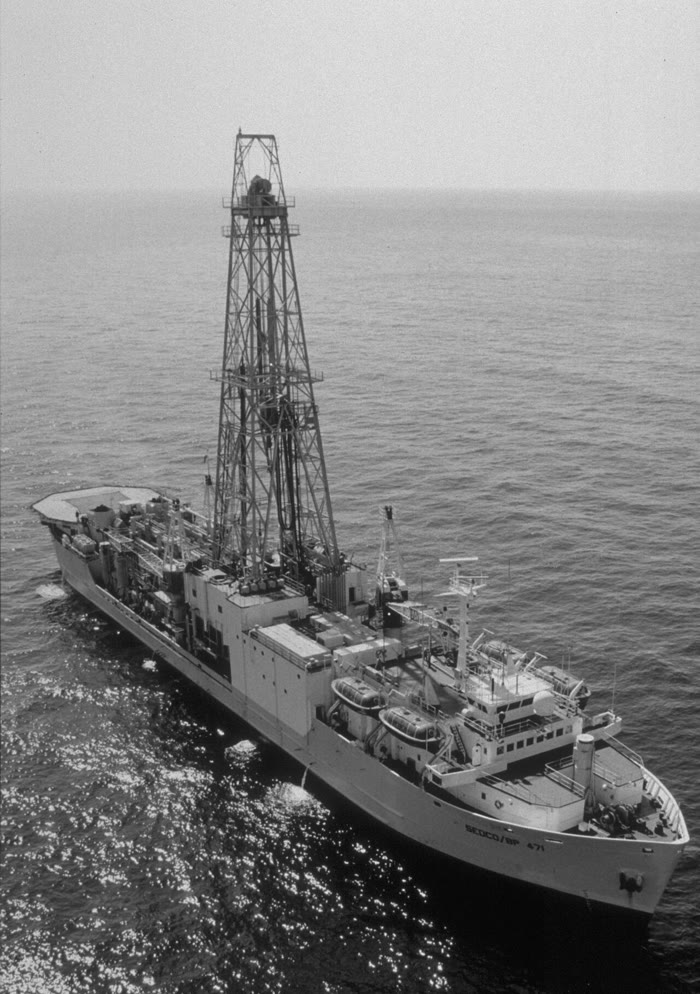
\includegraphics[width=0.36\linewidth]{images/book2/g11-odp-joides-resolution.jpg}

{\small Le navire de forage \emph{JOIDES Resolution}, qui a succédé au
\emph{Glomar Challenger}~: la haute tour est son derrick de forage, et le
navire emporte plus de \qty{9000}{m} de tiges de forage. Photographie~:
Ocean Drilling Program, Texas A\&M University (domaine public).}
\end{omfigure}
% ledger: photo:g11-joides, usgs:glomar

Depuis, des milliers de profils magnétiques et des centaines de forages ont
été réunis en une carte de l'âge de l'ensemble du fond océanique.

\begin{omfigure}
\begin{tikzpicture}
\begin{axis}[ommap, width=\linewidth, xtick=\empty, ytick=\empty, grid=none,
    axis background/.style={}, clip=true, name=map]
  \addplot graphics[xmin=-180, xmax=180, ymin=-90, ymax=90] {figdata/out/grade-11-seafloor_age.png};
  \addplot[black!60, line width=0.15pt] table {figdata/out/shared-geo-land.dat};
\end{axis}
\begin{axis}[at={(map.south)}, anchor=north, yshift=-0.35cm, scale only axis, width=0.55\linewidth, height=0.32cm,
    xmin=0, xmax=200, ymin=0, ymax=1, axis y line=none, axis x line*=bottom,
    xtick={0,20,...,180}, tick label style={font=\scriptsize},
    xlabel={âge du fond océanique (millions d'années)~; en gris~: pas de fond océanique}, label style={font=\scriptsize},
    enlargelimits=false]
  \addplot graphics[xmin=0, xmax=200, ymin=0, ymax=1] {figdata/out/grade-11-seafloor_age-bar.png};
\end{axis}
\end{tikzpicture}

{\small L'âge du fond océanique. Plus jeune (en rouge) le long des dorsales,
il vieillit en s'en éloignant des deux côtés~; le fond le plus ancien (en
bleu et violet) se trouve au bord des océans, contre les continents et le
long des fosses. Données~: Seton et ses collègues (2020), en cellules de
1~degré~; contours des terres~: Natural Earth.}
\end{omfigure}
% ledger: data:b2-seafloor-age, data:ne-land (map computed in figdata/grade-11/seafloor_age.py)

La carte confirme tout à la fois. Le long de chaque dorsale, le fond est
jeune, et son âge croît symétriquement en s'en éloignant. Aucun fond
océanique n'a plus de \num{190}~millions d'années environ~: le plus ancien
se trouve dans le Pacifique Ouest et au large de la côte est de l'Amérique
du Nord (quelques petits bassins de la Méditerranée orientale sont comptés
à part). L'âge moyen du fond océanique est d'environ \num{64}~millions
d'années, et environ les trois quarts ont moins de 100~millions
d'années --- alors que les continents conservent des roches bien plus
anciennes. Le fond océanique est jeune parce qu'il se forme sans cesse aux
dorsales et, comme l'avait vu Hess, qu'il est détruit ailleurs~: où, c'est
l'objet du \cref{ch:g11:subduction-zones}.
% ledger: data:b2-seafloor-age (oldest_open_myr 192.5, share_younger_100 0.76 in figdata/grade-11/seafloor_age.py), seton:mean-age, usgs:hess

\section{Exercices}

\begin{exercise}[$\star$]\label{exo:g11:drift-to-spreading:1}
Définir l'\omterm{def:g11:drift-to-spreading:spreading}{expansion des fonds océaniques}. Quelle est la différence entre la
\omterm{def:g11:drift-to-spreading:spreading-rate}{vitesse d'expansion totale} et la demi-vitesse d'expansion d'une dorsale~?
\end{exercise}

\begin{exercise}[$\star$]\label{exo:g11:drift-to-spreading:2}
Pourquoi une lave n'enregistre-t-elle la direction du champ terrestre
qu'une fois refroidie sous environ \qty{580}{\celsius}~? Que devient cet
enregistrement si la roche est plus tard chauffée à \qty{700}{\celsius}~?
\end{exercise}

\begin{exercise}[$\star$]\label{exo:g11:drift-to-spreading:3}
Un échosondeur entend l'écho de son impulsion \qty{5.2}{s} après l'avoir
émise. En prenant pour vitesse du son dans l'eau de mer \qty{1500}{m/s},
quelle est la profondeur du fond~?
\end{exercise}

\begin{exercise}[$\star$]\label{exo:g11:drift-to-spreading:4}
Sur l'échelle des inversions de ce chapitre~: depuis combien de temps dure
l'intervalle normal actuel~? Combien de temps a duré l'événement de
Jaramillo~? Combien d'inversions se sont produites au cours des cinq
derniers millions d'années~?
\end{exercise}

\begin{exercise}[$\star$]\label{exo:g11:drift-to-spreading:5}
Les dorsales médio-océaniques sont longues d'environ \qty{65000}{km}. La
circonférence de la Terre est d'environ \qty{40000}{km}. Combien de fois
les dorsales feraient-elles le tour de la Terre~?
\end{exercise}

\begin{exercise}[$\star\star$]\label{exo:g11:drift-to-spreading:6}
Sur un profil magnétique, la limite entre les intervalles de Brunhes et de
Matuyama (\num{0.78}~million d'années) se trouve à \qty{20}{km} de l'axe de
la dorsale. Calculer la demi-vitesse et la vitesse totale en centimètres
par an.
\end{exercise}

\begin{exercise}[$\star\star$]\label{exo:g11:drift-to-spreading:7}
Sur un autre profil, la limite Gauss--Gilbert (\num{3.58}~millions
d'années) se trouve à \qty{45}{km} à l'ouest et à \qty{44}{km} à l'est de
l'axe. Calculer la demi-vitesse de chaque côté et la vitesse totale.
L'expansion est-elle symétrique~?
\end{exercise}

\begin{exercise}[$\star\star$]\label{exo:g11:drift-to-spreading:8}
Le site 19 du forage de 1968 se trouve à \qty{990}{km} de l'axe de la
dorsale médio-atlantique. Avec une demi-vitesse de \qty{1.9}{cm} par an,
prévoir l'âge du fond à cet endroit, et le comparer aux \num{49}~millions
d'années de son sédiment le plus ancien.
\end{exercise}

\begin{exercise}[$\star\star$]\label{exo:g11:drift-to-spreading:9}
Une dorsale s'ouvre à une demi-vitesse de \qty{2}{cm} par an. À l'aide de
l'échelle des inversions de ce chapitre, donner les distances à l'axe des
limites à 0.78, 0.99, 1.07, 1.77 et 1.95~million d'années, et dessiner les
bandes d'un côté, les normales en noir.
\end{exercise}

\begin{exercise}[$\star\star$]\label{exo:g11:drift-to-spreading:10}
L'âge moyen du fond océanique est d'environ \num{64}~millions d'années~; la
Terre a environ \num{4.6}~milliards d'années. Quelle fraction de l'âge de
la Terre cela représente-t-il~? Lequel des arguments de Hess cela
appuie-t-il~?
\end{exercise}

\begin{exercise}[$\star\star$]\label{exo:g11:drift-to-spreading:11}
Expliquer, à l'aide d'un dessin, pourquoi le motif des bandes magnétiques
d'un côté d'une dorsale est l'image miroir du motif de l'autre côté.
Qu'est-ce qui romprait cette symétrie~?
\end{exercise}

\begin{exercise}[$\star\star\star$]\label{exo:g11:drift-to-spreading:12}
On suppose que les dorsales, longues de \qty{65000}{km} en tout, s'ouvrent
à une vitesse totale moyenne de \qty{5}{cm} par an.
\begin{enumerate}
  \item Quelle surface de nouveau fond océanique forment-elles chaque
        année, en \unit{km^2}~?
  \item Le fond océanique couvre environ \qty{2.9e8}{km^2}. Combien de
        temps faudrait-il aux dorsales pour en former autant~?
  \item Comparer au fond océanique le plus ancien, d'environ
        \num{190}~millions d'années. Que doit-il arriver au fond océanique
        aussi vite qu'il se forme~?
\end{enumerate}
\end{exercise}

\begin{exercise}[$\star\star\star$]\label{exo:g11:drift-to-spreading:13}
L'événement de Jaramillo a duré de \num{0.99} à \num{1.07}~million
d'années. Quelle est la largeur de sa bande de chaque côté d'une dorsale de
demi-vitesse \qty{1.25}{cm} par an, et d'une dorsale de \qty{7.5}{cm} par
an~? La roche aimantée se trouve à environ \qty{3}{km} sous la surface de
la mer. Expliquer pourquoi l'événement apparaît nettement sur le profil
rapide de ce chapitre mais presque pas sur le profil lent.
\end{exercise}

\begin{exercise}[$\star\star\star$]\label{exo:g11:drift-to-spreading:14}
Aux sites de 1968, les sédiments sont épais de \qty{176}{m} au site 16,
dont le fond a environ \num{11}~millions d'années, et de \qty{72}{m}
seulement au site 20, vieux d'environ \num{67}~millions d'années. Calculer
la vitesse moyenne d'accumulation des sédiments à chaque site, en mètres par
million d'années. Peut-on dater le fond par l'épaisseur des sédiments~?
Qu'utilise-t-on à la place~?
\end{exercise}

\begin{exercise}[$\star\star\star$]\label{exo:g11:drift-to-spreading:15}
Sur un profil à travers une dorsale, la limite de \num{2.581}~millions
d'années se trouve à \qty{58}{km} à l'ouest et à \qty{70}{km} à l'est de
l'axe.
\begin{enumerate}
  \item Calculer la demi-vitesse de chaque côté et la vitesse totale.
  \item Le fond à l'est de l'axe s'est formé plus vite que le fond à
        l'ouest. Après 10~millions d'années à ces vitesses, à quelle
        distance de l'axe se trouverait le fond de cet âge de chaque côté~?
  \item Expliquer pourquoi la distance entre les deux limites donne la
        vitesse totale même si l'expansion n'est pas symétrique.
\end{enumerate}
\end{exercise}

\section{Problème~: l'âge de l'Atlantique Sud}

\begin{problem}[{Problème du week-end --- dater un océan de trois façons}]
\label{pb:g11:drift-to-spreading:1}
% ledger: dsdp3:table5, dsdp3:rate, data:b2-seafloor-age, earth:Rmean, ics:base.Cretaceous
% (values computed in figdata/grade-11/sediment_ages.py and seafloor_age.py)
En 1968, le \emph{Glomar Challenger} fora sept trous à travers la dorsale
médio-atlantique près de la latitude \ang{30} Sud. Le tableau donne, pour
chaque site, sa distance à l'axe de la dorsale, l'âge du sédiment le plus
ancien reposant sur le basalte (d'après ses fossiles) et, quand la bande
située dessous a été identifiée, l'âge de cette bande magnétique, en
millions d'années.

\begin{center}
\small
\begin{tabular}{|c|c|c|c|}
\hline
site & distance à l'axe (\unit{km}) & âge du sédiment le plus ancien & âge de la bande magnétique \\ \hline
16 & 191 & 11 & 9 \\ \hline
15 & 380 & 24 & 21 \\ \hline
18 & 506 & 26 & --- \\ \hline
17 & 643 & 33 & --- \\ \hline
14 & 727 & 40 & 38.5 \\ \hline
19 & 990 & 49 & 53 \\ \hline
20 & 1270 & 67 & 71 \\ \hline
\end{tabular}

{\small Données~: Deep Sea Drilling Project, Leg 3 (1970)~; les âges
magnétiques sont le milieu des intervalles qui y sont donnés.}
\end{center}

\begin{center}
\begin{tikzpicture}
\begin{axis}[omrecord, width=0.82\linewidth, height=5.0cm, xmin=-50, xmax=16, ymin=0, ymax=140,
  xlabel={longitude le long de \ang{30} Sud (degrés~; négatif~: ouest)}, ylabel={âge (millions d'années)},
  tick label style={font=\small}, label style={font=\small}, clip=false]
\addplot[omDef, line width=0.8pt] table[x=lon, y=age] {figdata/out/grade-11-seafloor_age-profile.dat};
\draw[omRidge, densely dashed] (axis cs:-13.8,0) -- (axis cs:-13.8,140);
\node[font=\scriptsize, text=omRidge, anchor=south] at (axis cs:-13.8,140) {axe de la dorsale};
\fill (axis cs:-47.4,125.1) circle (1.5pt);
\node[font=\scriptsize, anchor=south west, inner sep=2pt] at (axis cs:-47.6,126) {Amérique du Sud};
\node[font=\scriptsize, anchor=north west, align=left] at (axis cs:14.2,135) {Afrique};
\fill (axis cs:13.8,129.8) circle (1.5pt);
\end{axis}
\end{tikzpicture}

{\small L'âge du fond océanique le long du parallèle \ang{30} Sud, de
l'Amérique du Sud à l'Afrique~; la courbe s'arrête là où le fond océanique
prend fin contre chaque continent. Données~: Seton et ses collègues (2020).}
\end{center}

\medskip
\noindent\textbf{Partie I --- Les sites de forage.}
\begin{enumerate}
  \item Quel site est le plus proche de la dorsale, et lequel le plus
        éloigné~? Comment leurs âges se comparent-ils~?
  \item Pourquoi l'âge du sédiment le plus ancien reposant sur le basalte
        est-il proche de l'âge du basalte lui-même~? Est-il un peu plus
        ancien ou un peu plus jeune~?
  \item Pour chaque site, calculer le rapport de sa distance à l'âge de son
        sédiment le plus ancien, en kilomètres par million d'années.
  \item Quelle est la moyenne de ces sept rapports~? La convertir en
        centimètres par an.
  \item Les sites 17 et 18 se trouvent à l'est de la dorsale, les autres à
        l'ouest. Les sites de l'est suivent-ils la même tendance que ceux de
        l'ouest~? Qu'est-ce que cela indique sur l'expansion~?
\end{enumerate}

\medskip
\noindent\textbf{Partie II --- La vitesse d'après les sédiments.}
\begin{enumerate}[resume]
  \item Si le fond s'était ouvert à une demi-vitesse constante $u$, comment
        l'âge $t$ du fond dépendrait-il de sa distance $d$ à l'axe~?
  \item La droite passant par l'origine qui ajuste le mieux les points a
        pour pente $u = \sum d\,t / \sum t^2$. Pour les sept sites,
        $\sum d\,t = \num{208276}$ et $\sum t^2 = \num{10952}$ (en
        kilomètres et en millions d'années). Calculer $u$ en kilomètres par
        million d'années et en centimètres par an.
  \item Quelle est la \omterm{def:g11:drift-to-spreading:spreading-rate}{vitesse d'expansion totale} de l'Atlantique Sud à
        cette latitude~?
  \item Les scientifiques de l'expédition ont écrit que la vitesse était
        «~un peu inférieure à \qty{2}{cm} par an~». Êtes-vous d'accord~?
  \item Avec cette vitesse, prévoir l'âge du fond au site 20, et le
        comparer à son sédiment le plus ancien.
\end{enumerate}

\medskip
\noindent\textbf{Partie III --- La vitesse d'après les bandes magnétiques.}
\begin{enumerate}[resume]
  \item À partir du seul site 16 (\qty{191}{km}, bande de 9~millions
        d'années), calculer une demi-vitesse.
  \item À partir du seul site 20 (\qty{1270}{km}, bande de 71~millions
        d'années), calculer une demi-vitesse.
  \item Pour les cinq sites qui ont un âge magnétique,
        $\sum d\,t = \num{180329}$ et
        $\sum t^2 = \num{9854}$. Calculer la meilleure demi-vitesse.
  \item De combien de pour cent les vitesses tirées des fossiles et des
        bandes diffèrent-elles~? Les deux méthodes concordent-elles~?
  \item Pourquoi est-il important que les deux âges aient été obtenus par
        des méthodes complètement différentes~?
\end{enumerate}

\medskip
\noindent\textbf{Partie IV --- Jusqu'au bord de l'océan.}
\begin{enumerate}[resume]
  \item Le long de \ang{30} Sud, l'axe de la dorsale se trouve à la
        longitude \ang{13.8} Ouest et le fond océanique prend fin contre
        l'Afrique à \ang{13.8} Est. Combien de degrés de longitude les
        séparent~?
  \item Sur une sphère de rayon \qty{6371}{km}, un degré de longitude
        mesure $\qty{111.2}{km} \times \cos(\text{latitude})$. Calculer la
        longueur d'un degré à \ang{30} Sud, et la distance de l'axe au bord
        du fond océanique près de l'Afrique.
  \item Si le fond s'était toujours ouvert à la vitesse de la partie~II,
        il y a combien de temps le fond du bord se serait-il formé~?
  \item La carte des âges, qui date le fond ancien par ses bandes
        magnétiques, donne \num{130}~millions d'années au bord. Quelle
        demi-vitesse moyenne cela implique-t-il~? L'ouverture précoce de
        l'océan a-t-elle été un peu plus rapide ou un peu plus lente que
        celle des 66 derniers millions d'années~?
  \item Conclure~: quel âge a le fond océanique le plus ancien près de
        l'Afrique à \ang{30} Sud~? Le Crétacé a commencé il y a environ
        \num{143}~millions d'années~: au cours de quelle période
        l'Atlantique Sud a-t-il commencé à s'ouvrir à cet endroit~?
\end{enumerate}
\end{problem}
